% Shell icon: postMode — wireframe isometric cube with triangulated faces
% (an FE mesh), the Post-Processing mode glyph. Same cube footprint as
% preMode.tex so the two toggle icons align optically.
\documentclass[tikz,border=2mm]{standalone}
\usetikzlibrary{arrows.meta,calc,shapes.geometric}
\begin{document}
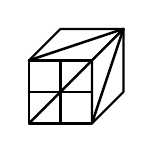
\begin{tikzpicture}[line width=1.3pt, line cap=round, line join=round, >=Stealth, x=1mm,y=1mm]
  % Cube outline (front rectangle, top + side parallelograms).
  \draw[thick] (-6,-8) rectangle (2,0);
  \draw[thick] (-6,0) -- (2,0) -- (6,4) -- (-2,4) -- cycle;
  \draw[thick] (2,-8) -- (6,-4) -- (6,4) -- (2,0) -- cycle;
  % Triangulation: one diagonal per face plus front-face midlines.
  \draw[line width=0.9pt] (-6,-8) -- (2,0);
  \draw[line width=0.9pt] (-6,-4) -- (2,-4);
  \draw[line width=0.9pt] (-2,-8) -- (-2,0);
  \draw[line width=0.9pt] (-6,0) -- (6,4);
  \draw[line width=0.9pt] (2,-8) -- (6,4);
\end{tikzpicture}
\end{document}
